\documentclass[tikz,border=10pt]{standalone}
\usetikzlibrary{shapes.geometric, arrows.meta}

\tikzset{
    block/.style={rectangle, draw, fill=blue!20, text width=6em, text centered, rounded corners, minimum height=3em},
    line/.style={draw, thick, -Stealth},
    connector/.style={thick, ->, >=stealth}
}

\begin{document}
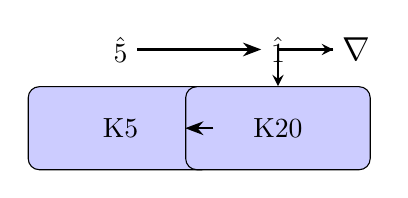
\begin{tikzpicture}[node distance=2cm]

    % Nodes for K5 and K20
    \node[block] (K5) {K5};
    \node[block, right of=K5] (K20) {K20};

    % Nodes for the hats
    \node[above of=K5, yshift=-1cm] (h5) {$\hat{5}$};
    \node[above of=K20, yshift=-1cm] (h1) {$\hat{1}$};

    % Nodes for the nabla symbol
    \node[right of=h5, xshift=1cm] (nabla) {\large $\nabla$};

    % Lines connecting nodes
    \draw[line] (K5) -- node[anchor=east] {$\overleftrightarrow{}$} (K20);
    \draw[line] (h5) -- (h1);
    \draw[connector] (h1) |- (nabla);
    \draw[connector] (nabla) -| (K20);

\end{tikzpicture}
\end{document}